\documentclass[11pt,a4paper]{article}

% ------------------------------------------------------------------ %
%  imrestore: technical note (software companion document)
%  Version 0.1.0, October 2026
% ------------------------------------------------------------------ %

\usepackage[american]{babel}
\usepackage[utf8]{inputenc}
\usepackage[T1]{fontenc}
\usepackage{amsmath,amssymb}
\usepackage{booktabs}
\usepackage[margin=2.5cm]{geometry}
\usepackage[numbers,sort&compress]{natbib}
\usepackage{graphicx}
\usepackage{algorithm}
\usepackage{algpseudocode}
\usepackage{hyperref}
\usepackage{enumitem}
\usepackage{xcolor}
\usepackage{abstract}
\usepackage[section]{placeins}
\usepackage[skip=6pt]{caption}

\graphicspath{{../figures/}}
\hypersetup{
  colorlinks=true,
  linkcolor=blue!40!black,
  citecolor=blue!40!black,
  urlcolor=blue!40!black,
}
\setlist{nosep}
\setlength{\emergencystretch}{3em}

\newcommand{\seprule}{\vspace{4pt}\noindent\rule{\textwidth}{0.5pt}\vspace{4pt}}
\newcommand{\code}[1]{\texttt{#1}}
\newcommand{\prox}{\operatorname{prox}}

\begin{document}
\sloppy

\begin{center}
{\LARGE\bfseries\texttt{imrestore}}\\[6pt]
{\Large\bfseries Adaptive and Quasi-Newton First-Order Methods\\[2pt]
 for Image Restoration}\\[10pt]
{\large Technical note}\\[10pt]
{\large Abd'gafar Tunde Tiamiyu}\\[4pt]
{\small School of Mathematics, Jilin University\\[2pt]
 Changchun 130012, Jilin, China}\\[4pt]
{\small\texttt{abdgafartunde@yahoo.com}}\\[12pt]
{\small\bfseries Version 0.1.0, October 2026}\\[4pt]
\seprule
\end{center}

\renewcommand{\abstractname}{Summary}
\begin{abstract}
\noindent
\texttt{imrestore} is an open-source Python package of first-order
optimization methods that need no hand-tuned step size, applied to image
denoising and deblurring. It implements adaptive gradient descent
(AdGD)~\cite{MalitskyMishchenko2020}, inertial quasi-Newton forward-backward
splitting (QN-FBS) with a rank-one metric~\cite{WangFadiliOchs2022}, and the
primal-dual algorithm with linesearch (PDAL)~\cite{MalitskyPock2018} with its
variable-metric extension (VarPDAL)~\cite{WangFadiliOchs2024}, together with
a Gaussian-blur operator, a total-variation operator, proximal maps, and
image-quality metrics. All methods are independent reimplementations from the
papers. This note states the problems each method solves, gives the
algorithms as implemented with their parameters and stopping rules, reports
the verification and restoration results, gives guidance on choosing the
parameters, and states the limitations. A step-by-step tutorial is provided
separately as \code{examples/00\_getting\_started.ipynb}.
\end{abstract}

\tableofcontents

% ================================================================== %
\section{Introduction}
% ================================================================== %

Image restoration recovers an image $x$ from a degraded observation
$b = Ax + n$, where $A$ is the identity (denoising) or a blur (deblurring)
and $n$ is noise. The standard approach is variational: minimize a data term
plus a regularizer, possibly with constraints such as $x\in[0,1]^N$. The
resulting problems take one of three forms, each served by one method:
\begin{center}
\begin{tabular}{lll}
\toprule
problem & method & module in \code{algorithms} \\
\midrule
$\min_x f(x)$, $f$ smooth & AdGD & \code{adaptive\_gd} \\
$0\in Az+Bz$, $B$ cocoercive & QN-FBS & \code{quasi\_newton\_fbs} \\
$\min_x\max_y \langle Kx,y\rangle + g(x) + h(x) - f^*(y)$ & PDAL, VarPDAL &
\code{var\_pdal} \\
\bottomrule
\end{tabular}
\end{center}
None of the methods needs the Lipschitz constant of a gradient or the norm of
an operator to be known in advance: AdGD estimates the local curvature, and
PDAL and VarPDAL find their step sizes by linesearch. QN-FBS and VarPDAL add
a rank-one quasi-Newton correction to the metric of the proximal step.

\texttt{imrestore} depends only on NumPy, SciPy, and Matplotlib. It is
intended for comparing these methods on common problems and as a readable
reference implementation.

\paragraph{Installation.} From the repository root,
\code{pip install -e ".[dev]"} installs the package with the test and
notebook dependencies; \code{uv sync --extra dev} reproduces the exact
environment recorded in \code{uv.lock}.

% ================================================================== %
\section{Operators and proximal maps}
% ================================================================== %

\paragraph{Gaussian blur.} \code{GaussianBlur(sigma, kernel\_size)}
convolves with a normalized Gaussian kernel of size
$2\,\mathrm{round}(3\sigma)+1$ by default, as a \emph{circular} convolution
computed with the FFT. With periodic boundaries the symmetric kernel makes
the operator self-adjoint (\code{adjoint} returns the same convolution), and
because the kernel is nonnegative and sums to one, $\|A\|\le1$.

\paragraph{Discrete gradient and total variation.}
\code{TotalVariation(weight)} provides the forward-difference gradient
$D:\mathbb R^{n_r\times n_c}\to\mathbb R^{2\times n_r\times n_c}$ with zero
differences across the last row and column (\code{forward}), its exact
adjoint, which is minus the divergence (\code{adjoint}), the isotropic TV
value $w\sum_{ij}|(Dx)_{ij}|$ (\code{\_\_call\_\_}), and the projection onto
the dual ball $\{p:|p_{ij}|\le w\}$ (\code{prox\_conj}), which is the
proximal map of the conjugate of $w\|\cdot\|_{2,1}$. Since TV has no simple
proximal map of its own, TV problems are solved in the primal-dual form with
$K=D$.

\paragraph{Proximal maps.} \code{operators.proximal} provides
soft-thresholding (\code{prox\_l1}), shrinkage (\code{prox\_l2\_squared}),
and projection onto a box (\code{prox\_box}); the first two accept a
diagonal metric.

% ================================================================== %
\section{Algorithms}
% ================================================================== %

Every solver returns an \code{OptimizationResult} with the final iterate
\code{x}, the objective history (when an \code{objective} callable is given;
it is used for diagnostics only), the step-size history, and the number of
iterations \code{n\_iter}.

\subsection{Adaptive gradient descent}

\code{adaptive\_gradient\_descent(gradient, x0, objective, lambda\_0,
max\_iter, tol)} implements Algorithm~1 of~\cite{MalitskyMishchenko2020}
(Algorithm~\ref{alg:adgd}). The step size combines growth by at most
$\sqrt{1+\theta}$ with a local estimate of the inverse curvature from the
last two iterates and gradients. If $f$ is convex with a locally Lipschitz
gradient, the iterates converge to a minimizer and a weighted average of
them achieves $f-f_*=O(1/k)$; under local strong convexity the convergence
is linear~\cite{MalitskyMishchenko2020}. The method stops when
$\|\nabla f(x^k)\|\le\code{tol}$.

\code{accelerated\_adaptive\_gradient\_descent} implements the paper's
accelerated variant (Algorithm~2), which also estimates the local
strong-convexity constant and adds momentum. The paper presents it as a
heuristic without a convergence proof.

\begin{algorithm}[ht]
\caption{AdGD (\code{adaptive\_gradient\_descent})}
\label{alg:adgd}
\begin{algorithmic}[1]
\Require $x^0$, $\lambda_0>0$ (default $10^{-10}$); $\theta_0=+\infty$
\State $x^1 = x^0 - \lambda_0\nabla f(x^0)$
\For{$k=1,2,\dots$}
  \State $\lambda_k = \min\Bigl\{\sqrt{1+\theta_{k-1}}\,\lambda_{k-1},\
    \dfrac{\|x^k-x^{k-1}\|}{2\|\nabla f(x^k)-\nabla f(x^{k-1})\|}\Bigr\}$
  \Comment{second term dropped if the denominator is zero}
  \State $x^{k+1} = x^k - \lambda_k\nabla f(x^k)$;
    \quad $\theta_k = \lambda_k/\lambda_{k-1}$
\EndFor
\end{algorithmic}
\end{algorithm}

\subsection{Inertial quasi-Newton forward-backward splitting}

\code{inertial\_quasi\_newton\_fbs(B, resolvent\_A, z0, beta, theta0,
inertial\_alpha, gamma, objective, max\_iter, tol)} solves the monotone
inclusion $0\in Az+Bz$, where $B$ is $\beta$-cocoercive (for example
$B=\nabla f$ with $f$ convex and $L$-smooth, $\beta=1/L$) and $A$ is
maximally monotone with a simple resolvent in a scalar metric (for
$A=\partial g$, \code{resolvent\_A(v, theta)} $=\prox_{g/\theta}(v)$). It
implements Algorithm~1 of~\cite{WangFadiliOchs2022} with the base metric
$M_0=\theta_0I$, $\theta_0>1/\beta$ (default $1.1/\beta$), and a single
rank-one correction per iteration (the paper's 0SR1 update, Section~5):
\begin{equation}\label{eq:0sr1}
  M_k = \theta_0 I \pm \gamma_k\,u_ku_k^\top,\qquad
  u_k = \frac{r_k}{\sqrt{|\langle r_k,s_k\rangle|}},\quad
  r_k = y_k-\theta_0s_k,
\end{equation}
with $s_k = z_k - z_{k-1}$, $y_k = Bz_k - Bz_{k-1}$, the sign of
$\langle r_k,s_k\rangle$, and no update when that inner product vanishes.
For the minus sign, $\gamma_k$ is clipped so that $M_k$ stays positive
definite.

Each iteration takes an inertial step
$\bar z_k = z_k + \alpha(z_k-z_{k-1})$, a forward step in the metric $M_0$,
and a backward step in the metric $M_k$. The latter is computed by the
paper's resolvent calculus: it reduces to finding the root of a strictly
increasing scalar function, found by bracketing (up to 40 expansions) and
bisection (60 steps), with two evaluations of the simple resolvent per step;
$M_k$ is never formed or inverted. The method stops when
$\|z_{k+1}-z_k\|\le\code{tol}$.

The paper's convergence theorem requires a summable-type inertial schedule.
A constant \code{inertial\_alpha}$>0$ is a common heuristic that the
theorem does not cover; \code{inertial\_alpha = 0} (the default) runs the
non-inertial method, which it does.

\subsection{PDAL and VarPDAL}

Both solve the saddle-point problem
\begin{equation}\label{eq:saddle}
  \min_x\max_y\ \langle Kx,y\rangle + g(x) + h(x) - f^*(y)
\end{equation}
with $g$ and $f^*$ simple (prox-friendly) and $K$ linear. For TV
restoration, $K=D$, $f^*$ is the indicator of the dual ball
(\code{TotalVariation.prox\_conj}), $g$ is the indicator of the box
$[0,1]^N$ (\code{prox\_box}), and $h(x)=\tfrac12\|Ax-b\|^2$ is the data term.

\paragraph{PDAL.} \code{pdal(K, K\_adjoint, prox\_g, prox\_f\_conj, x0,
y1, tau0, beta, mu, delta, objective, max\_iter, tol, max\_linesearch)}
implements Algorithm~1 of~\cite{MalitskyPock2018} for $h\equiv0$
(Algorithm~\ref{alg:pdal}). It replaces the condition $\sigma\tau\|K\|^2<1$
by a backtracking linesearch on the primal step, with the dual step
$\beta\tau_k$.

\begin{algorithm}[ht]
\caption{PDAL (\code{pdal})}
\label{alg:pdal}
\begin{algorithmic}[1]
\Require $x^0$, $y^1$, $\tau_0>0$, $\beta>0$, $\mu,\delta\in(0,1)$ (defaults
0.7, 0.99); $\theta_0=1$
\For{$k=1,2,\dots$}
  \State $x^k = \prox_{\tau_{k-1}g}\bigl(x^{k-1}-\tau_{k-1}K^*y^k\bigr)$
  \State $\tau_k = \tau_{k-1}\sqrt{1+\theta_{k-1}}$
  \Repeat \Comment{at most \code{max\_linesearch} times}
    \State $\theta_k=\tau_k/\tau_{k-1}$;\quad
      $\bar x^k = x^k + \theta_k(x^k-x^{k-1})$
    \State $y^{k+1} = \prox_{\beta\tau_kf^*}\bigl(y^k+\beta\tau_kK\bar x^k\bigr)$
    \State \textbf{if} $\sqrt\beta\,\tau_k\|K^*y^{k+1}-K^*y^k\|\le
      \delta\|y^{k+1}-y^k\|$ \textbf{then break}; \textbf{else}
      $\tau_k\gets\mu\tau_k$
  \Until{accepted}
  \State stop if $\|x^k-x^{k-1}\|+\|y^{k+1}-y^k\|\le\code{tol}$
\EndFor
\end{algorithmic}
\end{algorithm}

\paragraph{VarPDAL.} \code{var\_pdal(K, K\_adjoint, prox\_g, prox\_f\_conj,
h, grad\_h, x1, y0, L\_h, sigma0, beta, theta0, gamma, mu, delta, objective,
max\_iter, tol, max\_linesearch)} implements Algorithm~1
of~\cite{WangFadiliOchs2024} for the full problem~\eqref{eq:saddle} with
$h$ convex and $\nabla h$ $L_h$-Lipschitz. It linesearches the dual step
$\sigma_k$ (with $\tau_k=\beta\sigma_k$) and takes the primal proximal step
in a quasi-Newton metric $M_k$:
\[
  x^{k+1} = \prox^{M_k}_{\tau_kg}\bigl(x^k - \tau_kM_k^{-1}(K^*\bar y^k +
  \nabla h(x^k))\bigr),
\]
accepting $\sigma_k$ when
\[
  \tau_k\sigma_k\|Kx^{k+1}-Kx^k\|^2 + 2\tau_k\bigl(h(x^{k+1})-h(x^k)-
  \langle\nabla h(x^k),x^{k+1}-x^k\rangle\bigr) \le
  \delta\|x^{k+1}-x^k\|^2_{M_k},
\]
and shrinking it by $\mu$ otherwise. The paper's default metric is a
multi-memory L-BFGS/L-SR1 metric with a semismooth-Newton resolvent; for
consistency and $O(N)$ cost, \texttt{imrestore} uses instead the rank-one
metric~\eqref{eq:0sr1} and the scalar resolvent calculus of QN-FBS, with
secant pairs from consecutive values of $\nabla h$ and
$\theta_0>L_h$ (default $1.1L_h$). It stops when the change in the primal
and dual iterates is at most \code{tol}.

% ================================================================== %
\section{Verification}
% ================================================================== %

\begin{figure}[!h]
\centering
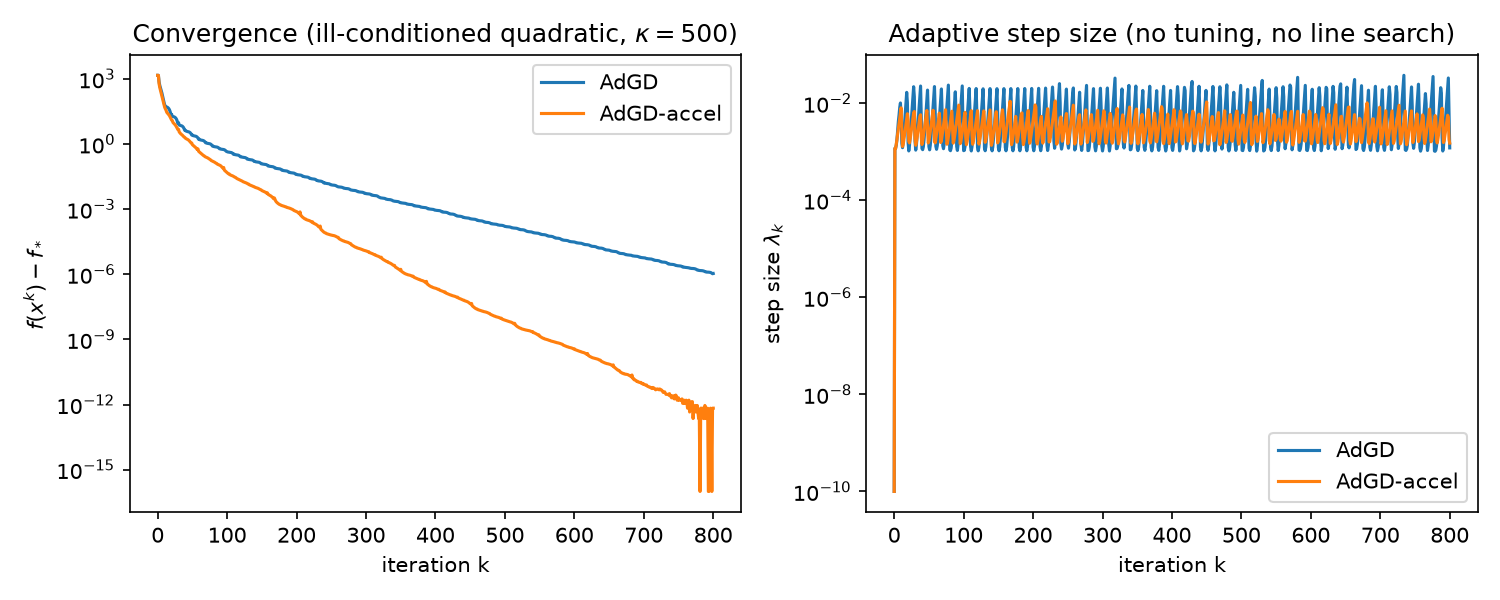
\includegraphics[width=0.32\textwidth]{adaptive_gd_convergence.png}\hfill
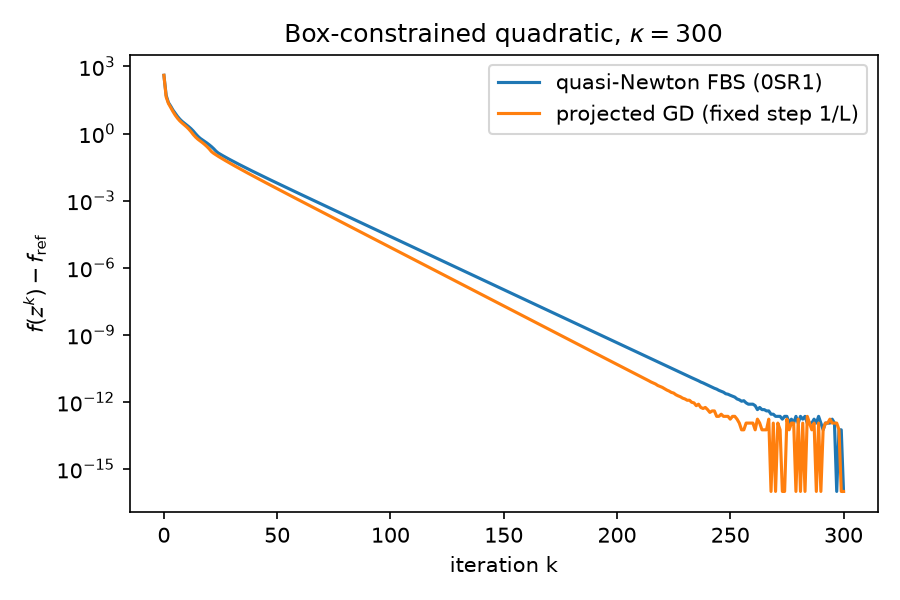
\includegraphics[width=0.32\textwidth]{quasi_newton_fbs_convergence.png}\hfill
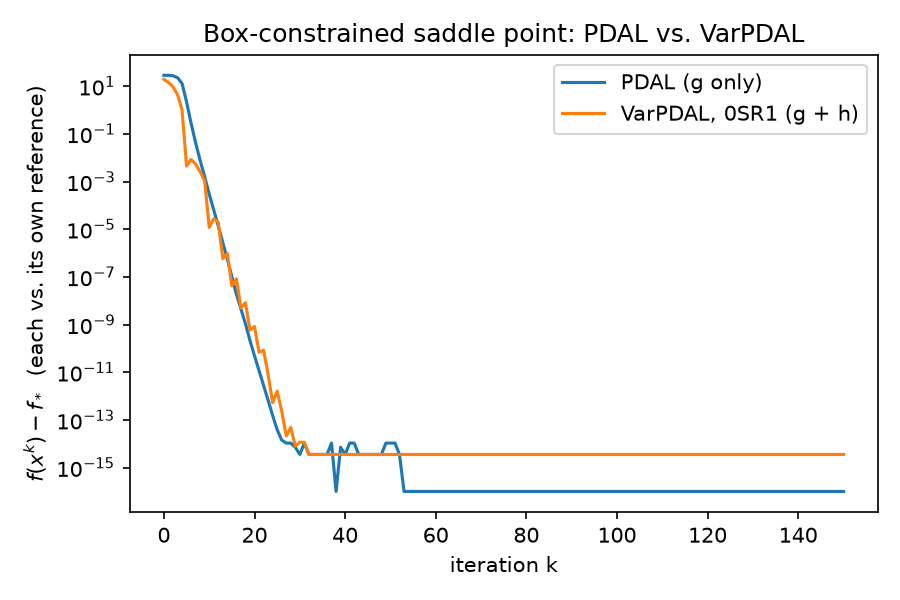
\includegraphics[width=0.32\textwidth]{var_pdal_convergence.png}
\caption{Algorithm demos on synthetic problems. Left: AdGD and its
accelerated variant on a quadratic with condition number 500. Centre: QN-FBS
against projected gradient descent with step $1/L$ on a box-constrained
quadratic with condition number 300. Right: PDAL and VarPDAL on a
box-constrained saddle-point problem, each against its own closed-form
reference.}
\label{fig:demos}
\end{figure}

\begin{itemize}
  \item \emph{Operators.} For random inputs, the blur and the discrete
        gradient pass the dot-product test
        $\langle Au,v\rangle=\langle u,A^*v\rangle$ to twelve digits; the blur
        preserves constant images and rejects kernels larger than the image.
  \item \emph{Proximal maps.} \code{prox\_l1} matches the closed form and
        satisfies the optimality condition; \code{prox\_l2\_squared} and
        \code{prox\_box} match their closed forms; \code{prox\_conj} projects
        onto the dual ball.
  \item \emph{Solvers.} Each solver converges to the known minimizer of a test
        problem: AdGD and its accelerated variant on quadratics (the variant
        needs fewer iterations on an ill-conditioned one), QN-FBS on an
        unconstrained and a box-constrained quadratic (with and without
        inertia), PDAL on a saddle-point problem with a closed-form
        solution, and VarPDAL on the same problem with an added smooth term.
        Invalid parameters ($\theta_0\le1/\beta$, $\theta_0\le L_h$) are
        rejected.
  \item \emph{Convergence demos.} \code{scripts/demo\_*.py} compare each
        method with a baseline on synthetic problems with closed-form
        references (Figure~\ref{fig:demos}).
\end{itemize}
The test suite has 31 tests. Continuous integration runs it on Python 3.10
to 3.13, runs every script from outside the repository, and executes both
notebooks; the benchmark notebook reproduces its stored outputs exactly.

% ================================================================== %
\section{Restoration results}
% ================================================================== %

All results use the $96\times96$ Shepp--Logan phantom with values in
$[0,1]$.

\paragraph{TV restoration with VarPDAL.} \code{scripts/restoration\_demo.py}
runs two experiments (Figures~\ref{fig:denoise} and~\ref{fig:deblur}):
\begin{itemize}
  \item denoising with noise $\sigma=0.08$ and TV weight $w=0.1$, 200
        iterations: PSNR 23.6 to 25.8\,dB, SSIM 0.40 to 0.62;
  \item deblurring a Gaussian blur with $\sigma=1$ and noise $\sigma=0.01$,
        with $w=10^{-3}$ and 3000 iterations: PSNR 19.7 to 29.3\,dB, SSIM
        0.76 to 0.93.
\end{itemize}
Both weights favour visual quality over PSNR. For denoising, PSNR peaks at
$w=0.05$ (27.8\,dB) and SSIM at $w=0.07$ (0.631); $w=0.1$ gives flatter
regions at 25.8\,dB and SSIM 0.623. For deblurring, a sweep with the same
settings gives PSNR 30.8\,dB at $w=3\times10^{-4}$ to $5\times10^{-4}$ and
29.3\,dB at $10^{-3}$, while SSIM peaks at $10^{-3}$ (0.927).

\begin{figure}[ht]
\centering
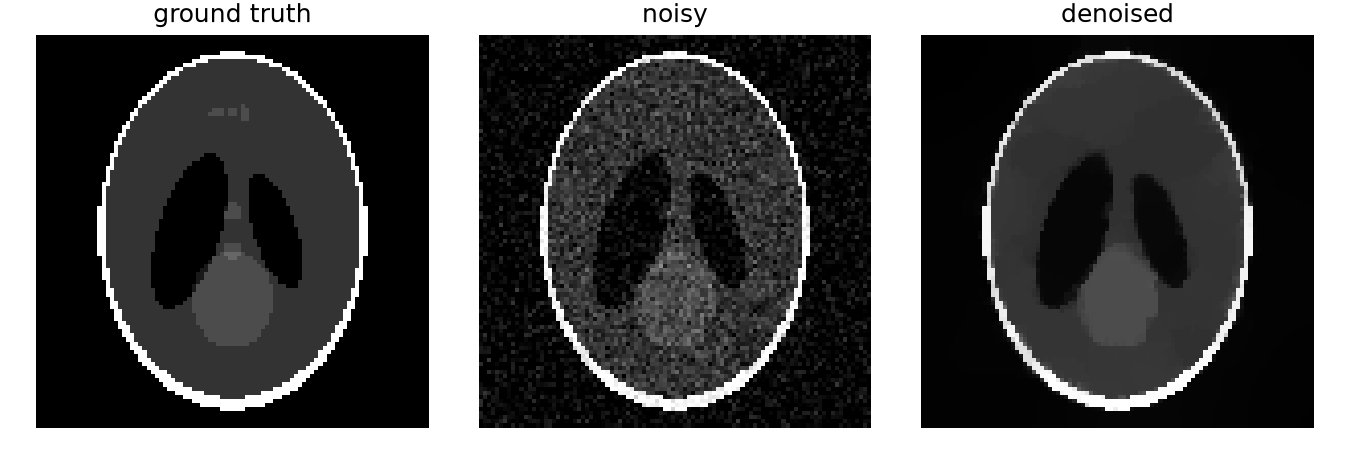
\includegraphics[width=0.9\textwidth]{restoration_denoising.png}
\caption{TV denoising with VarPDAL ($\sigma=0.08$, $w=0.1$).}
\label{fig:denoise}
\end{figure}

\begin{figure}[ht]
\centering
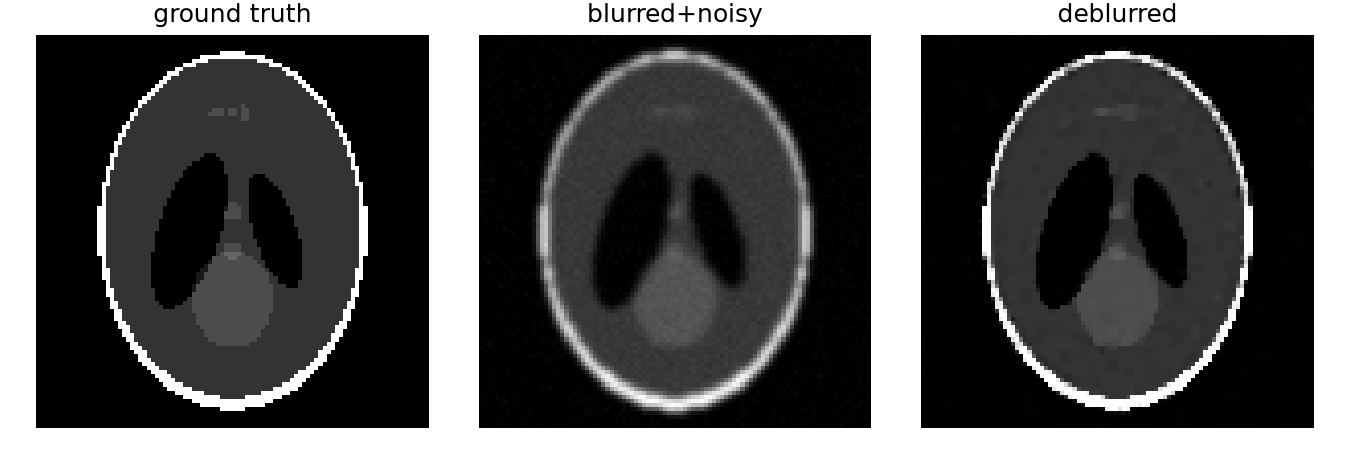
\includegraphics[width=0.9\textwidth]{restoration_deblurring.png}
\caption{TV deblurring with VarPDAL (blur $\sigma=1$, noise $0.01$,
$w=10^{-3}$).}
\label{fig:deblur}
\end{figure}

\paragraph{The three methods on denoising.} The benchmark notebook
(\code{examples/01\_restoration\_benchmark.ipynb}) denoises with noise
$\sigma=0.12$ (PSNR 20.19\,dB, SSIM 0.320). AdGD and QN-FBS minimize a
smooth Tikhonov objective with a gradient penalty (QN-FBS adds the box
constraint) and reach 21.34\,dB (SSIM 0.350) in 38 and 30 iterations;
VarPDAL with TV ($w=0.08$, 200 iterations) reaches 24.40\,dB (SSIM 0.562).

\paragraph{Step sizes.} In the tutorial's deblurring problem with a smooth
objective ($L\le1.08$), AdGD reaches machine precision in about 200
iterations, while gradient descent with the fixed step $1/L$ is still near
$10^{-10}$ after 300. Its median step is 1.76, about twice $1/L$, and its
largest is 17.6.

\paragraph{Choosing the TV weight.} In the tutorial (deblurring without
clipping the data), the discrepancy principle~\cite{Morozov1966}, which picks
the weight whose residual $\|Ax_w-b\|$ matches the noise norm
$\sigma\sqrt N$, selects $w=10^{-3}$ (PSNR 29.3\,dB, SSIM 0.963, the highest
SSIM in the sweep); the PSNR optimum is at $w=3\times10^{-4}$ (30.9\,dB).
VarPDAL with 3000 iterations takes about 5\,s at this size on an Apple
M-series laptop.

% ================================================================== %
\section{Choosing the parameters}
% ================================================================== %

\paragraph{AdGD.} Leave \code{lambda\_0} at its default; the step grows to
the local curvature scale within a few iterations. Set \code{tol} on the
gradient norm, and pass \code{objective} only to record the history.

\paragraph{QN-FBS.} Pass the cocoercivity constant \code{beta} $=1/L$ of
$B$; for $f(x)=\tfrac12\|Ax-b\|^2+\tfrac\mu2\|Dx\|^2$ with the blur and
gradient above, $L\le\|A\|^2+8\mu\le1+8\mu$. Keep
\code{inertial\_alpha = 0} if you need the convergence guarantee.

\paragraph{PDAL and VarPDAL.} The initial step (\code{tau0} or
\code{sigma0}) only needs to be of the right order: the linesearch adjusts
it. The ratio \code{beta} between primal and dual steps matters more;
\code{beta = 1} works for TV restoration with images in $[0,1]$. For
VarPDAL pass $L_h=\|A\|^2$, which is at most 1 for the normalized blur.
Small TV weights make the problem close to unregularized deblurring and need
thousands of iterations; check that the result no longer changes when
\code{max\_iter} is doubled.

\paragraph{Regularization weight.} Use the discrepancy principle when the
noise level is known, and compare the images as well as PSNR and SSIM, which
can disagree for TV.

% ================================================================== %
\section{Software reference}
% ================================================================== %

\begin{table}[ht]
\centering
\small
\caption{Public functions (module prefixes relative to \code{imrestore}).}
\begin{tabular}{@{}p{0.52\textwidth}p{0.43\textwidth}@{}}
\toprule
function & purpose \\
\midrule
\code{algorithms.adaptive\_gd}:\newline \code{adaptive\_gradient\_descent},\newline
\code{accelerated\_adaptive\_gradient\_descent} & AdGD and its accelerated
  variant \\
\code{algorithms.quasi\_newton\_fbs}:\newline
\code{inertial\_quasi\_newton\_fbs} & QN-FBS with the 0SR1 metric \\
\code{algorithms.var\_pdal}:\newline \code{pdal}, \code{var\_pdal} & PDAL and VarPDAL \\
\code{operators.blur.GaussianBlur(sigma, kernel\_size)} & periodic Gaussian
  blur \\
\code{operators.tv.TotalVariation(weight)} & gradient, adjoint, TV value,
  dual projection \\
\code{operators.proximal.prox\_l1}, \code{prox\_l2\_squared},
  \code{prox\_box} & proximal maps \\
\code{metrics.image\_quality.psnr}, \code{ssim} & PSNR and SSIM (data range
  1 by default) \\
\code{utils.io.load\_phantom(name, size)}, \code{add\_gaussian\_noise}
  & test images (\code{"shepp-logan"}, \code{"circles"}) and noise \\
\code{utils.visualization.plot\_convergence},
  \code{plot\_restoration\_grid} & plotting \\
\bottomrule
\end{tabular}
\end{table}

\paragraph{Reproducing the results.} The figures in this note are in
\code{figures/} and are regenerated by the scripts in \code{scripts/},
which run from any directory and accept \code{--outdir}.

% ================================================================== %
\section{Limitations}
% ================================================================== %

\begin{itemize}
  \item \emph{Metrics.} QN-FBS and VarPDAL use a rank-one quasi-Newton
        metric only; the multi-memory L-BFGS/L-SR1 metrics of the papers are
        not implemented.
  \item \emph{Guarantees.} The accelerated AdGD variant and QN-FBS with a
        constant inertial parameter are heuristics without the papers'
        guarantees; the accelerated variants of PDAL are not implemented.
  \item \emph{Models.} Grayscale images, Gaussian blur with periodic
        boundaries, and Gaussian noise; no Poisson data terms, no
        spatially varying blur.
  \item \emph{Implementation.} Pure NumPy on the CPU.
\end{itemize}

% ================================================================== %
\begin{thebibliography}{99}
% ================================================================== %

\bibitem{MalitskyMishchenko2020}
Y.~Malitsky and K.~Mishchenko.
\newblock Adaptive gradient descent without descent.
\newblock In \emph{Proceedings of the 37th International Conference on
  Machine Learning (ICML)}, PMLR 119, 2020.
\newblock arXiv:1910.09529.

\bibitem{MalitskyPock2018}
Y.~Malitsky and T.~Pock.
\newblock A first-order primal-dual algorithm with linesearch.
\newblock \emph{SIAM Journal on Optimization}, 28(1):411--432, 2018.

\bibitem{Morozov1966}
V.A.~Morozov.
\newblock On the solution of functional equations by the method of
  regularization.
\newblock \emph{Soviet Mathematics Doklady}, 7:414--417, 1966.

\bibitem{WangFadiliOchs2022}
S.~Wang, J.~Fadili, and P.~Ochs.
\newblock Inertial quasi-Newton methods for monotone inclusion: efficient
  resolvent calculus and primal-dual methods.
\newblock arXiv:2209.14019, 2022 (v3, 2024).
\newblock See also: Quasi-Newton methods for monotone inclusions: efficient
  resolvent calculus and primal-dual algorithms, \emph{SIAM Journal on
  Imaging Sciences}, 18(1):308--344, 2025.

\bibitem{WangFadiliOchs2024}
S.~Wang, J.~Fadili, and P.~Ochs.
\newblock A quasi-Newton primal-dual algorithm with line search.
\newblock arXiv:2405.06824, 2024.
\newblock See also the conference paper with the same title in
  \emph{Scale Space and Variational Methods in Computer Vision}, Lecture
  Notes in Computer Science, pages 444--456, Springer, 2023.

\end{thebibliography}

\end{document}
